\documentclass[10pt]{beamer}

\usetheme[progressbar=frametitle]{metropolis}
\usepackage{appendixnumberbeamer}

\usepackage{booktabs}
\usepackage[scale=2]{ccicons}

\usepackage{pgfplots}
\usepgfplotslibrary{dateplot}

\usepackage{xspace}
\newcommand{\themename}{\textbf{\textsc{metropolis}}\xspace}

\title{A Glimpse into Quantum-enhanced Machine Learning Solutions}

\date{\today}

\author{
	Massimiliano Pronesti, 
	Federico Tiblias, 
	Giulio Corallo
}

\institute{Amadeus Knowledge Sharing Session}


\begin{document}
	
	\maketitle
	
	\begin{frame}{Who are we?}

Three Computer Engineering and Data Science students interested in Machine Learning and fascinated by Quantum Computing
    
\end{frame}


	
	\begin{frame}{Table of contents}
		\setbeamertemplate{section in toc}[sections numbered]
		\tableofcontents
		%[hideallsubsections]
		% uncomment the above line to hide subsections
	\end{frame}
	
	%%% THIS IS HOW YOU IMPORT STUFF FROM OTHER FILES!!!!
	\section[Introduction]{Introduction}

\begin{frame}{Why Quantum?}
Imagine you want to seat 10 fussy people at a dinner party, where there is only one optimal seating plan out of all the different possible combinations. How many different combinations would you have to explore to find the optimal?

Can you guess how many \alert{combinations}?
\end{frame}

\begin{frame}{Why Quantum?}


			
			
		
			
			\metroset{block=fill}
			
			\begin{exampleblock}{For 2 people}
				2 Total combination.
			\end{exampleblock}
			
			\begin{block}{For 5 people}
				120 Total combination.
			\end{block}
			
			\begin{alertblock}{For 10 people}
				Over 3 Million of total combination!!!
			\end{alertblock}
			
		
				
				
			
			
			
\begin{itemize}
			\item Supercomputers don't have the working \alert{memory} to hold the myriad combinations of real world problems.
			\item Supercomputers have to analyze each combination one after another, which can take a long \alert{time}.
		\end{itemize}
		
				
				

\end{frame}

\begin{frame}[fragile]{Quantum Computers}
%Until now, we’ve relied on supercomputers to solve most problems. %These are very large classical computers, often with thousands of %classical CPU and GPU cores. However, supercomputers aren’t very %good at solving certain types of problems, which seem easy at first %glance. This is why we need quantum computers.
\begin{figure}[H]
  \centering
    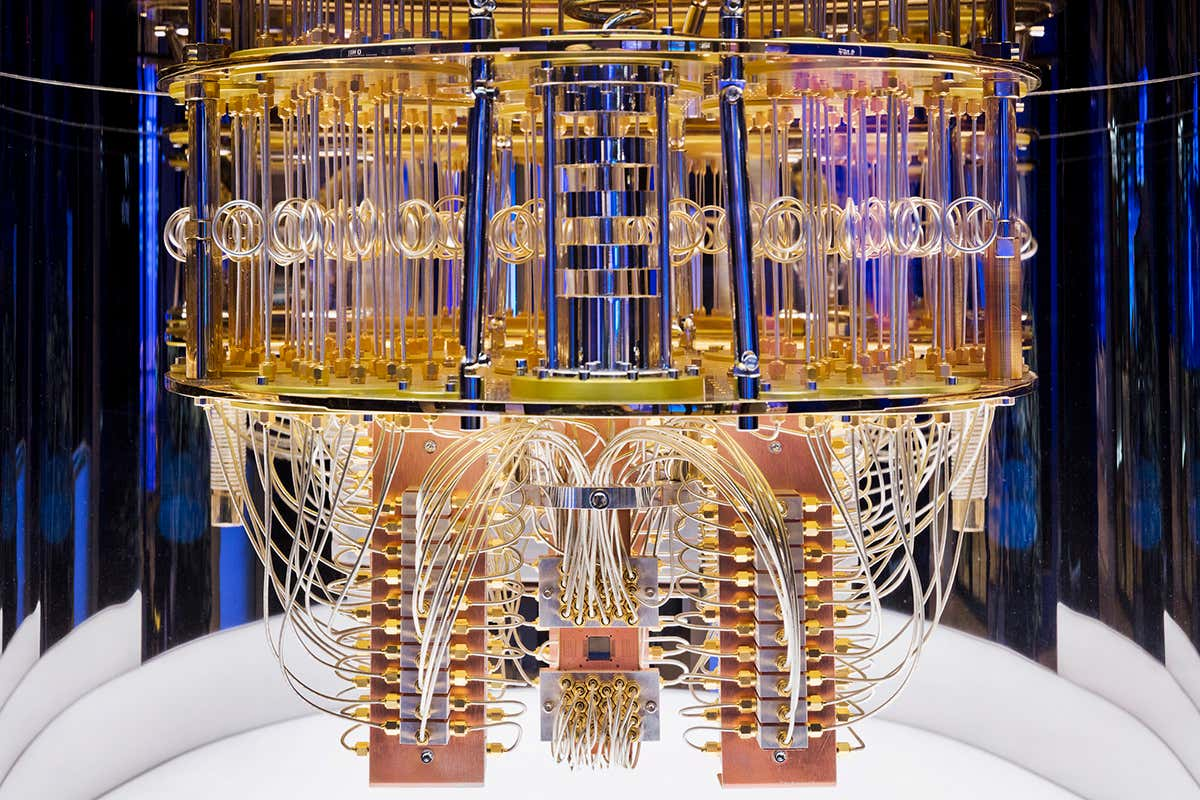
\includegraphics[width=.8\linewidth]{assets/quantum-computers-1.jpg}
    \caption{Quantum Computer}
\end{figure}

\end{frame}

\begin{frame}[fragile]{Metropolis}
	
	The \themename theme is a Beamer theme with minimal visual noise
	inspired by the \href{https://github.com/hsrmbeamertheme/hsrmbeamertheme}{\textsc{hsrm} Beamer
		Theme} by Benjamin Weiss.
	
	Enable the theme by loading
	
	\begin{verbatim}    \documentclass{beamer}
		\usetheme{metropolis}\end{verbatim}
	
	Note, that you have to have Mozilla's \emph{Fira Sans} font and XeTeX
	installed to enjoy this wonderful typography.
\end{frame}

\begin{frame}[fragile]{Sections}
	Sections group slides of the same topic
	
	\begin{verbatim}    \section{Elements}\end{verbatim}
	
	for which \themename provides a nice progress indicator \ldots
	
\end{frame}
	
	\begin{frame}{Bra-ket notation}
    Useful for representing quantum systems
		\begin{columns}[T,onlytextwidth]
			\column{0.5\textwidth}
			\centering
			Bra $=$ Row
			\begin{align*}
			    \langle A\rvert
			     = 
                \begin{bmatrix}
                a_{0} & a_{1} & a_{2} & \cdots
                \end{bmatrix}
            \end{align*}
			\column{0.5\textwidth}
			\centering
			Ket $=$ Column
            \begin{align*}
			    \lvert B\rangle
			     = 
                \begin{bmatrix}
                b_{0} \\
                b_{1} \\
                b_{2} \\
                \vdots \\
                \end{bmatrix}
            \end{align*}
		\end{columns}
		Properties & operations:
		\begin{itemize}
			\item Scalar product $= \langle A\lvert B \rangle = [a_{0}, a_{1}, a_{2}, \cdots] \cdot [b_{0}, b_{1}, b_{2}, \cdots]^T$ 
			\item Norm $= \langle A\lvert A \rangle = |A|^2$
		\end{itemize}
    
\end{frame}


	
	\begin{frame}{What is a qubit?}

		\begin{itemize}
			\item Building block for quantum computers
			\item 2-state quantum system (photon, electron, Schrodinger's cat, ...)
			\item 0, 1, both at the same time (superposition)
			\item Can be manipulated (quantum circuits)
			\item Can form more complex quantum systems (multi-quibit systems)
			\item Can be observed causing its collapse (measurement)
		\end{itemize}
		
		\begin{figure}[H]
          \centering
            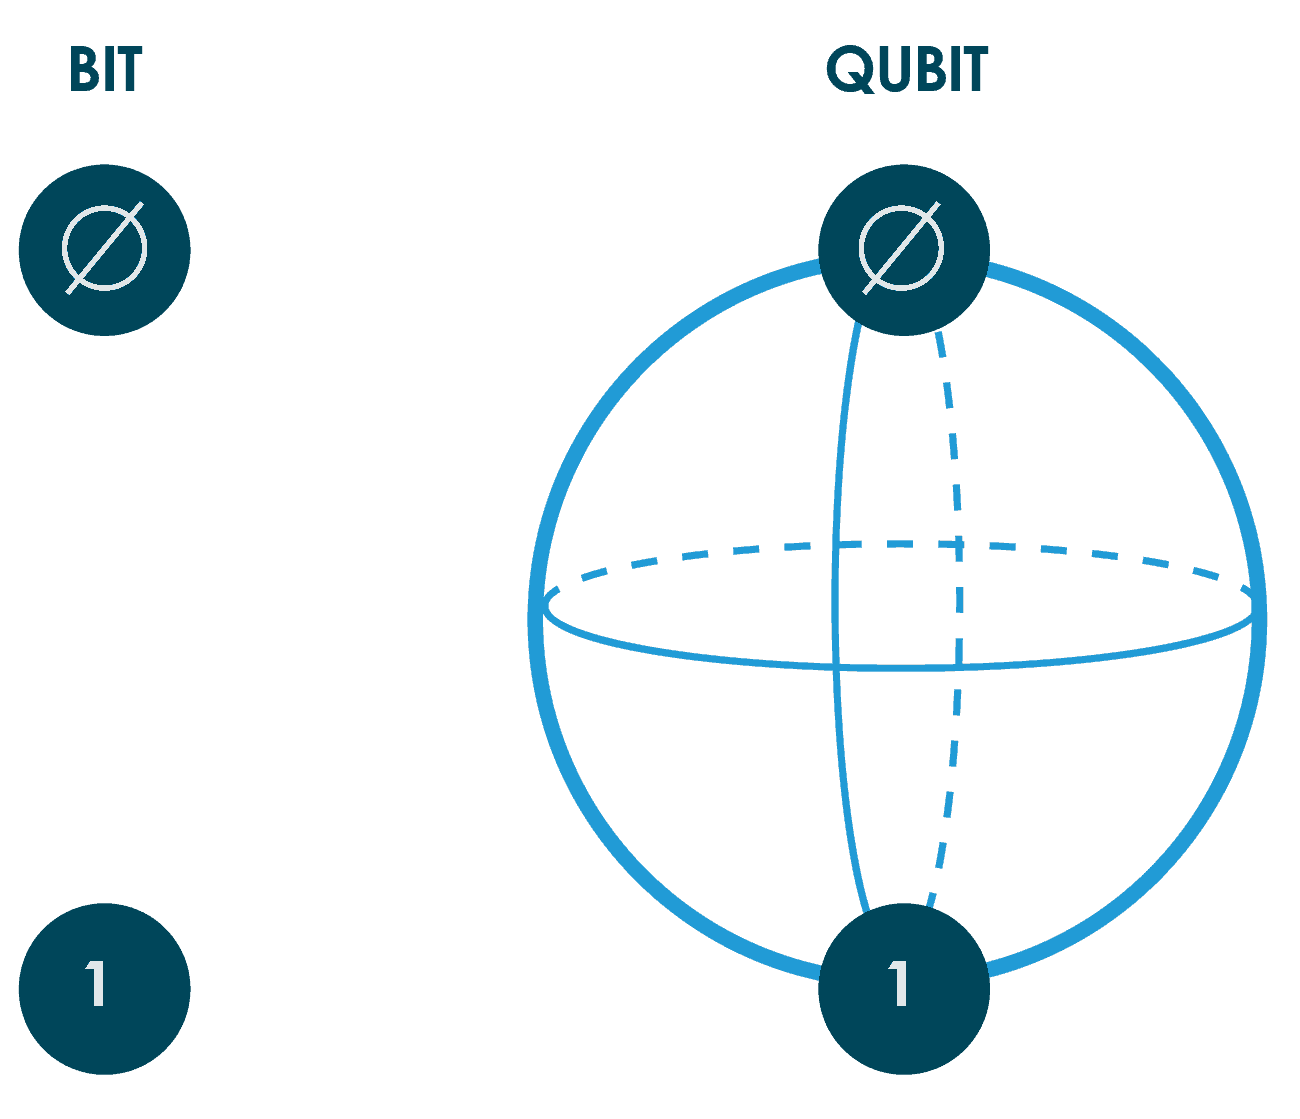
\includegraphics[width=.4\linewidth]{assets/Qubit.png}
        \end{figure}
    
\end{frame}

\begin{frame}{What is a qubit?}
		\begin{itemize}
			\item What does it mean to be 0 and 1 simultaneously?
			
			    It's a matter of probability during measurement
			
            \item Bra-ket qubit representation:
            \begin{columns}[T,onlytextwidth]
			\column{0.33\textwidth}
			\centering
			\begin{align*}
			    \lvert 0\rangle
			     = 
                \begin{bmatrix}
                1 \\
                0
                \end{bmatrix}
            \end{align*}
			
			\column{0.33\textwidth}
			\centering
            \begin{align*}
			    \lvert 1\rangle
			    = 
                \begin{bmatrix}
                0 \\
                1
                \end{bmatrix}
            \end{align*}
            
            \column{0.33\textwidth}
			\centering
            \begin{align*}
			    \lvert \psi\rangle
			    = 
                \begin{bmatrix}
                \psi_0 \\
                \psi_1
                \end{bmatrix}
            \end{align*}
		\end{columns}
		
		
		\item Probability measurement:
		    \begin{align*}
			    P(\lvert \psi\rangle = 0) = \lvert\psi_0\rvert^2
			\end{align*}
			\begin{align*}
			    P(\lvert \psi\rangle = 1) = \lvert\psi_1\rvert^2
            \end{align*}
		\item Probability distribution: $\langle \psi\lvert \psi \rangle = |\psi|^2 = 1 \ \forall \ \psi$

        \end{itemize}
\end{frame}

\begin{frame}{Multi-qubit system and entanglement}
    How can we represent 2 or more qubits with bra-kets? 
    
    With tensor products and longer vectors
    \begin{align*}
	    \lvert AB\rangle
		=
		\begin{bmatrix}
        a_0 \\       
        a_1 \\
        \end{bmatrix}
		\otimes
        \begin{bmatrix}
        b_0 \\       
        b_1 \\
        \end{bmatrix}
        =
        \begin{bmatrix}
        a_0 b_0 \\
        a_0 b_1 \\
        a_1 b_0 \\
        a_1 b_1 \\
        \end{bmatrix}
    \end{align*}
    By stacking $n$ qubits we can represent $2^n$ infinite precision numbers
    
    \centering
    $P(A = 0, B = 1) = \lvert a_0 b_1 \rvert^2 $
\end{frame}


\begin{frame}{Multi-qubit system and entanglement}
    How can we represent state $\lvert 00\rangle + \lvert 11\rangle $ with a tensor product? 
    
    We can't as there is no set of values for $a_0, a_1, b_0, b_1$ that allows it.
    \begin{align*}
	    \lvert AB\rangle
		=
		\begin{bmatrix}
        a_0 b_0 \\
        a_0 b_1 \\
        a_1 b_0 \\
        a_1 b_1 \\
        \end{bmatrix}
    \end{align*}
    
    However, we can still create this state with quantum circuits. The resulting state is said to be entangled as measuring one qubit immediately tells us the state of the other.
    \begin{align*}
	    \lvert 00\rangle + \lvert 11\rangle 
		=
		\begin{bmatrix}
        1/\sqrt{2} \\
        0 \\
        0 \\
        1/\sqrt{2} \\
        \end{bmatrix}
    \end{align*}
\end{frame}
	%%%%%%%%%%%%%%%%%%%%%%%%%%%%%%%%%%%%%%%%%%%%%%%%%%%%%%%%%%%%%%%%%%
	%%% DA QUA IN POI NON LO STO FACENDO PIÙ PER NON PERDERE
	%%% TEMPO A SPOSTARE COSE CHE TANTO SONO SOLO ESEMPI DEL TEMPLATE
	%%% PERO' OGNI SEZIONE DEVE STARE IN UN FILE A PARTE!!
	%%%%%%%%%%%%%%%%%%%%%%%%%%%%%%%%%%%%%%%%%%%%%%%%%%%%%%%%%%%%%%%%%%
	
	\section{Titleformats}
	
	\begin{frame}{Metropolis titleformats}
		\themename supports 4 different titleformats:
		\begin{itemize}
			\item Regular
			\item \textsc{Smallcaps}
			\item \textsc{allsmallcaps}
			\item ALLCAPS
		\end{itemize}
		They can either be set at once for every title type or individually.
	\end{frame}
	
	\subsection{Tricks}
	
	{
		\metroset{titleformat frame=smallcaps}
		\begin{frame}{Small caps}
			This frame uses the \texttt{smallcaps} titleformat.
			
			\begin{alertblock}{Potential Problems}
				Be aware, that not every font supports small caps. If for example you typeset your presentation with pdfTeX and the Computer Modern Sans Serif font, every text in smallcaps will be typeset with the Computer Modern Serif font instead.
			\end{alertblock}
		\end{frame}
	}
	
	{
		\metroset{titleformat frame=allsmallcaps}
		\begin{frame}{All small caps}
			This frame uses the \texttt{allsmallcaps} titleformat.
			
			\begin{alertblock}{Potential problems}
				As this titleformat also uses smallcaps you face the same problems as with the \texttt{smallcaps} titleformat. Additionally this format can cause some other problems. Please refer to the documentation if you consider using it.
				
				As a rule of thumb: Just use it for plaintext-only titles.
			\end{alertblock}
		\end{frame}
	}
	
	{
		\metroset{titleformat frame=allcaps}
		\begin{frame}{All caps}
			This frame uses the \texttt{allcaps} titleformat.
			
			\begin{alertblock}{Potential Problems}
				This titleformat is not as problematic as the \texttt{allsmallcaps} format, but basically suffers from the same deficiencies. So please have a look at the documentation if you want to use it.
			\end{alertblock}
		\end{frame}
	}
	
	\section{Elements}
	
	\begin{frame}[fragile]{Typography}
		\begin{verbatim}The theme provides sensible defaults to
			\emph{emphasize} text, \alert{accent} parts
			or show \textbf{bold} results.\end{verbatim}
		
		\begin{center}becomes\end{center}
		
		The theme provides sensible defaults to \emph{emphasize} text,
		\alert{accent} parts or show \textbf{bold} results.
	\end{frame}
	
	\begin{frame}{Font feature test}
		\begin{itemize}
			\item Regular
			\item \textit{Italic}
			\item \textsc{SmallCaps}
			\item \textbf{Bold}
			\item \textbf{\textit{Bold Italic}}
			\item \textbf{\textsc{Bold SmallCaps}}
			\item \texttt{Monospace}
			\item \texttt{\textit{Monospace Italic}}
			\item \texttt{\textbf{Monospace Bold}}
			\item \texttt{\textbf{\textit{Monospace Bold Italic}}}
		\end{itemize}
	\end{frame}
	
	\begin{frame}{Lists}
		\begin{columns}[T,onlytextwidth]
			\column{0.33\textwidth}
			Items
			\begin{itemize}
				\item Milk \item Eggs \item Potatos
			\end{itemize}
			
			\column{0.33\textwidth}
			Enumerations
			\begin{enumerate}
				\item First, \item Second and \item Last.
			\end{enumerate}
			
			\column{0.33\textwidth}
			Descriptions
			\begin{description}
				\item[PowerPoint] Meeh. \item[Beamer] Yeeeha.
			\end{description}
		\end{columns}
	\end{frame}
	\begin{frame}{Animation}
		\begin{itemize}[<+- | alert@+>]
			\item \alert<4>{This is\only<4>{ really} important}
			\item Now this
			\item And now this
		\end{itemize}
	\end{frame}
	\begin{frame}{Figures}
		\begin{figure}
			\newcounter{density}
			\setcounter{density}{20}
			\begin{tikzpicture}
				\def\couleur{alerted text.fg}
				\path[coordinate] (0,0)  coordinate(A)
				++( 90:5cm) coordinate(B)
				++(0:5cm) coordinate(C)
				++(-90:5cm) coordinate(D);
				\draw[fill=\couleur!\thedensity] (A) -- (B) -- (C) --(D) -- cycle;
				\foreach \x in {1,...,40}{%
					\pgfmathsetcounter{density}{\thedensity+20}
					\setcounter{density}{\thedensity}
					\path[coordinate] coordinate(X) at (A){};
					\path[coordinate] (A) -- (B) coordinate[pos=.10](A)
					-- (C) coordinate[pos=.10](B)
					-- (D) coordinate[pos=.10](C)
					-- (X) coordinate[pos=.10](D);
					\draw[fill=\couleur!\thedensity] (A)--(B)--(C)-- (D) -- cycle;
				}
			\end{tikzpicture}
			\caption{Rotated square from
				\href{http://www.texample.net/tikz/examples/rotated-polygons/}{texample.net}.}
		\end{figure}
	\end{frame}
	\begin{frame}{Tables}
		\begin{table}
			\caption{Largest cities in the world (source: Wikipedia)}
			\begin{tabular}{lr}
				\toprule
				City & Population\\
				\midrule
				Mexico City & 20,116,842\\
				Shanghai & 19,210,000\\
				Peking & 15,796,450\\
				Istanbul & 14,160,467\\
				\bottomrule
			\end{tabular}
		\end{table}
	\end{frame}
	\begin{frame}{Blocks}
		Three different block environments are pre-defined and may be styled with an
		optional background color.
		
		\begin{columns}[T,onlytextwidth]
			\column{0.5\textwidth}
			\begin{block}{Default}
				Block content.
			\end{block}
			
			\begin{alertblock}{Alert}
				Block content.
			\end{alertblock}
			
			\begin{exampleblock}{Example}
				Block content.
			\end{exampleblock}
			
			\column{0.5\textwidth}
			
			\metroset{block=fill}
			
			\begin{block}{Default}
				Block content.
			\end{block}
			
			\begin{alertblock}{Alert}
				Block content.
			\end{alertblock}
			
			\begin{exampleblock}{Example}
				Block content.
			\end{exampleblock}
			
		\end{columns}
	\end{frame}
	\begin{frame}{Math}
		\begin{equation*}
			e = \lim_{n\to \infty} \left(1 + \frac{1}{n}\right)^n
		\end{equation*}
	\end{frame}
	\begin{frame}{Line plots}
		\begin{figure}
			\begin{tikzpicture}
				\begin{axis}[
					mlineplot,
					width=0.9\textwidth,
					height=6cm,
					]
					
					\addplot {sin(deg(x))};
					\addplot+[samples=100] {sin(deg(2*x))};
					
				\end{axis}
			\end{tikzpicture}
		\end{figure}
	\end{frame}
	\begin{frame}{Bar charts}
		\begin{figure}
			\begin{tikzpicture}
				\begin{axis}[
					mbarplot,
					xlabel={Foo},
					ylabel={Bar},
					width=0.9\textwidth,
					height=6cm,
					]
					
					\addplot plot coordinates {(1, 20) (2, 25) (3, 22.4) (4, 12.4)};
					\addplot plot coordinates {(1, 18) (2, 24) (3, 23.5) (4, 13.2)};
					\addplot plot coordinates {(1, 10) (2, 19) (3, 25) (4, 15.2)};
					
					\legend{lorem, ipsum, dolor}
					
				\end{axis}
			\end{tikzpicture}
		\end{figure}
	\end{frame}
	\begin{frame}{Quotes}
		\begin{quote}
			Veni, Vidi, Vici
		\end{quote}
	\end{frame}
	
	{%
		\setbeamertemplate{frame footer}{My custom footer}
		\begin{frame}[fragile]{Frame footer}
			\themename defines a custom beamer template to add a text to the footer. It can be set via
			\begin{verbatim}\setbeamertemplate{frame footer}{My custom footer}\end{verbatim}
		\end{frame}
	}
	
	\begin{frame}{References}
		Some references to showcase [allowframebreaks] \cite{knuth92,ConcreteMath,Simpson,Er01,greenwade93}
	\end{frame}
	
	\section{Conclusion}
	
	\begin{frame}{Summary}
		
		All the material used for this presentation is available at the following link:
		
		\begin{center}
			\url{https://github.com/mspronesti/talk-qml-amadeus}
		\end{center}
		
		\begin{center}\ccbysa\end{center}
		
	\end{frame}
	
	
	%% Questions Slide
	{\setbeamercolor{palette primary}{fg=black}
		\begin{frame}[standout]
			Thanks for you attention!\\ Any Question ?
		\end{frame}
	}
	
	\appendix
	
	
	%% Bibliography
	\begin{frame}[allowframebreaks]{References}
		\bibliography{ref}
		\bibliographystyle{abbrv}
	\end{frame}
	
\end{document}
